% Template for PLoS
% Version 3.3 June 2016
%
% % % % % % % % % % % % % % % % % % % % % %
%
% -- IMPORTANT NOTE
%
% This template contains comments intended 
% to minimize problems and delays during our production 
% process. Please follow the template instructions
% whenever possible.
%
% % % % % % % % % % % % % % % % % % % % % % % %

% Created to hold supplementary information

\documentclass[10pt,letterpaper]{article}

\usepackage[top=0.85in,left=2in,footskip=0.75in]{geometry}

% amsmath and amssymb packages, useful for mathematical formulas and symbols
\usepackage{amsmath,amssymb}

% Use adjustwidth environment to exceed column width (see example table in text)
\usepackage{changepage}

% Use Unicode characters when possible
\usepackage[utf8x]{inputenc}

% textcomp package and marvosym package for additional characters
\usepackage{textcomp,marvosym}

% cite package, to clean up citations in the main text. Do not remove.
\usepackage{cite}

% Use nameref to cite supporting information files (see Supporting Information section for more info)
\usepackage{nameref,hyperref}

% line numbers
\usepackage[right]{lineno}

% ligatures disabled
\usepackage{microtype}
\DisableLigatures[f]{encoding = *, family = * }

% color can be used to apply background shading to table cells only
\usepackage[table]{xcolor}

% array package and thick rules for tables
\usepackage{array}

% create "+" rule type for thick vertical lines
\newcolumntype{+}{!{\vrule width 2pt}}


% create \thickcline for thick horizontal lines of variable length
\newlength\savedwidth
\newcommand\thickcline[1]{%
  \noalign{\global\savedwidth\arrayrulewidth\global\arrayrulewidth 2pt}%
  \cline{#1}%
  \noalign{\vskip\arrayrulewidth}%
  \noalign{\global\arrayrulewidth\savedwidth}%
}

% \thickhline command for thick horizontal lines that span the table
\newcommand\thickhline{\noalign{\global\savedwidth\arrayrulewidth\global\arrayrulewidth 2pt}%
\hline
\noalign{\global\arrayrulewidth\savedwidth}}


% Remove comment for double spacing
%\usepackage{setspace} 
%\doublespacing

% Text layout
\raggedright
\setlength{\parindent}{0.5cm}
\textwidth 5.25in 
\textheight 8.75in

% Bold the 'Figure #' in the caption and separate it from the title/caption with a period
% Captions will be left justified
\usepackage[aboveskip=1pt,labelfont=bf,labelsep=period,justification=raggedright,singlelinecheck=off]{caption}
\renewcommand{\figurename}{Fig}

% Use the PLoS provided BiBTeX style
\bibliographystyle{plos2015}

% Remove brackets from numbering in List of References
\makeatletter
\renewcommand{\@biblabel}[1]{\quad#1.}
\makeatother

% Leave date blank
\date{}

% Header and Footer with logo
\usepackage{lastpage,fancyhdr,graphicx}
\usepackage{epstopdf}
\pagestyle{myheadings}
\pagestyle{fancy}
\fancyhf{}
\setlength{\headheight}{27.023pt}
\lhead{
\includegraphics[width=3.0in]{PLOS-submission.eps}}
\rfoot{\thepage/\pageref{LastPage}}
\renewcommand{\footrule}{\hrule height 2pt \vspace{2mm}}
\fancyheadoffset[L]{1.25in}
\fancyfootoffset[L]{1.25in}
\lfoot{\sf PLOS}

%% Include all macros below

\newcommand{\lorem}{{\bf LOREM}}
\newcommand{\ipsum}{{\bf IPSUM}}

%% END MACROS SECTION

\begin{document}
\vspace*{0.2in}

% Title must be 250 characters or less.
\begin{flushleft}
{\Large
\textbf\newline{Research Synergy and Drug Development: Bright Stars in Neighboring Constellations} % Please use "title case" (capitalize all terms in the title except conjunctions, prepositions, and articles).
}
\newline
% Insert author names, affiliations and corresponding author email (do not include titles, positions, or degrees).
\\
Samet Keserci\textsuperscript{1},
%Samet Keserci\textsuperscript{1,2\Yinyang},
Eric Livingston\textsuperscript{2},
Lingtian Wan\textsuperscript{1,\textcurrency},
Alexander R. Pico\textsuperscript{3},
%Name5 Surname\textsuperscript{2\ddag},
%Name6 Surname\textsuperscript{2\ddag},
 \& George Chacko\textsuperscript{1*}
%with the Lorem Ipsum Consortium\textsuperscript{\textpilcrow}
\\
\bigskip
\textbf{1} Netelabs, NET ESolutions Corporation, McLean, VA, USA
\\
\textbf{2} Elsevier Research Intelligence, Elsevier Inc., Bethesda, MD, USA
\\
\textbf{3} Gladstone Institutes, University of California San Francisco, San Francisco, CA, USA
\\
\bigskip


% Insert additional author notes using the symbols described below. Insert symbol callouts after author names as necessary.
% 
% Remove or comment out the author notes below if they aren't used.
%
% Primary Equal Contribution Note
%\Yinyang These authors contributed equally to this work.

% Additional Equal Contribution Note
% Also use this double-dagger symbol for special authorship notes, such as senior authorship.
%\ddag These authors also contributed equally to this work.

% Current address notes
\textcurrency Current Address: Facebook Corporation, Menlo Park, CA, USA % change symbol to "\textcurrency a" if more than one current address note
% \textcurrency b Insert second current address 
% \textcurrency c Insert third current address

% Deceased author note
%\dag Deceased

% Group/Consortium Author Note
%\textpilcrow Membership list can be found in the Acknowledgments section.

% Use the asterisk to denote corresponding authorship and provide email address in note below.
*Correspondence: george@nete.com
\end{flushleft}
% Please keep the abstract below 300 words
\section*{Abstract}

Drug discovery and the subsequent availability of new breakthrough therapeutics or `cures' are compelling examples of societal benefit from advances in research. Such advances are invariably collaborative, involving the contributions of many scientists in a `cure network' where prior theory and experiment is built upon. To understand such scientific advances, data mining of public and commercial data sources coupled with network analysis can be used as a digital methodology to assemble component events in the history of a cure and analyze them. This methodology is extensible beyond cure networks and its use supports (i) efficiency in  exploring  the scientific history of a research advance (ii) documenting and understanding collaboration (iii) portfolio analysis, planning and optimization (iv) communication of the societal value of research.  As a proof of principle, we have conducted a case study of five anti-cancer therapeutics. For the purpose of exploring the relationship across networks, we have built upon a technique for single networks and linked the work of approximately 250,000 authors in 100,000 scientific publications, we have enriched the content of networks for these therapeutics by annotating them with information on research awards as well as peer review that preceded these awards. Applying retrospective citation discovery, we have identified a core set of publications cited in the networks of all five therapeutics and additional intersections in combinations of networks as well as a core set of awards from the National Institutes of Health that supported this research. Lastly, we have mapped these awards to their cognate peer review panels, identifying another layer of collaborative scientific activity that influenced the research represented by these networks. 

\linenumbers

\section*{Introduction}

Data mining of public data sources coupled with network analysis enables the assembly and quantitative description of research discoveries that were influential in the development of a breakthrough therapeutic or `cure'.  The set of scientific publications, clinical trials, patents, and regulatory approvals, linked to each other by citation or assignment, that documents the progress of concepts from basic research to a cure is termed a `cure network' \cite {bibWilliams}. Key assumptions in constructing these networks are that the references found in relevant documents are appropriate citations of new knowledge relevant to a given cure and that a further retrospective round of citation discovery will uncover previous influential discovery (\textit{ibid}). Beyond using a digital methodology to assemble a set of facts about a major scientific advance, however, these studies also support a contextual understanding of knowledge diffusion across disciplines, scientific interests, culture, and time\cite{bibMaldame}. Coupled with the knowledge that accrues from the clinical use of the drug, knowledge of a drug development network also enables a recursive learning of the pathogenesis of the disease it is being used to treat as as been noted for the burgeoning field of immunotherapeutics\cite{bibChan}. 

Such studies (i) provide evidence for the broad collaborative platform of basic and translational research underlying major scientific advances such as cures for diseases (ii) support strategic communications to oversight bodies, and (iii) help communicate the societal value of research\cite {bibLauer}. Williams and colleagues have elegantly demonstrated the feasibility and value of data mining and network analysis using, as case studies, ivacaftor and ipilimumab, approved for the treatment of cystic fibrosis and melanoma respectively (\textit{vide supra}). These authors observed that `the nature of a cure discovery network is complex and fundamentally collaborative', noting in the case of ivacaftor, that at least 7,067 scientists with 5,666 unique affiliations contributed to ivacaftor-related research over a period greater than 100 years. 

Extending this methodology to study additional cures and significant research advances in general is a logical next step. Ascertaining the nature of the interactions, if any, between networks, is also of considerable interest since it would support an understanding of collaboration across networks as well as common features of science networks. Lastly, scaling from case studies to mapping the entire domain of drug development may be beneficial in future resource allocation and optimization of drug development activities. 

To address these questions, we have enhanced prior art to (i) incorporate enhanced data mining methods and network metrics (ii) include enriched data from a commercially available bibliographic database with disambiguated author identifiers (iii) include information on research awards and peer review of grants (iv) extended single network analysis to map publications and authors across multiple networks (v) refactored the network analysis code of Williams et al. for better performance. To evaluate these extensions, we have conducted case studies of a cluster of five FDA-approved therapeutics for cancer. We present the results of this case study as a body of work for interrogation and improvement by other researchers, and a step towards mapping the universe of FDA-approved drugs and biologicals.

\section*{Materials and Methods}  A set of five anti-cancer therapeutics, three drugs and two biologicals, approved for use in humans by the Food and Drug Administration was selected for this study (Table 1). Imatinib and Sunitinib are tyrosine kinase inhibitors, Nelarabine is a nucleoside analog, and Ramucirumab and Alemtuzumab are humanized antibodies that target cell surface receptors. For each of these therapeutics, a set of relevant scientific publications was constructed as in Williams et al.\cite{bibWilliams} but with specific modifications detailed below. An allowance of 2 months was also made for `publication lag' when assembling referenced material. For example, if a therapeutic was approved on Jan 1, 2017, documents published  on or before March 31, 2017 were included. For each of the five therapeutics, a first-generation list of PubMed identifiers (citing\_pmid) was harvested from the five different data sources (below). 
 
\begin{table}[!ht]
%\begin{adjustwidth}{-0.5in}{0in} % Comment out/remove adjustwidth environment if table fits in text column.
\centering
\scalebox{0.9}{
\begin{tabular}{|l+l|l|l|l|l|l|l|}
\hline
%\multicolumn{4}{|l|}{\bf Heading1} & \multicolumn{4}{|l|}{\bf Heading2}\\ \thickhline
Therapeutic & FDA Approval Date & Unique Identifier & US Patent & Publication Date  \\ \hline
$Alemtuzumab$ & May 2001 & BLA: 103948 & US5846534 & Dec 1998\\ \hline
$Imatinib$ & May 2001 & NDA: 021335 & US5521184 &  May 1996 \\ \hline
$Nelarabine$ & Oct 2005 & NDA: 021877 & US5424295 & Jun 1995  \\ \hline
$Ramucirumab$ & Apr 2014 & BLA: 125477 & US7498414 & Mar 2009  \\ \hline
$Sunitinib$ & Jan 2006  & NDA: 021938  & US6573293 & Jun 2003 \\ \hline
\end{tabular}}
\vspace{2 mm}
\caption{
{\bf Case Studies of Five Anti-Cancer Agents} Five anti-cancer therapeutics, with FDA approval dates ranging from 2001 to 2014, were selected as case studies. The active ingredient for each of these five therapeutics is listed in column 1. While multiple patents are typically associated with a drug or biological, the single US patent number displayed represents the primary invention that preceded approval of the therapeutic. The publication date for each patent is listed in the last column.}
%\begin{flushleft}  
%\end{flushleft}
\label{table1}
%\end{adjustwidth}
\end{table}

\textbf{Clinical trials} The national clinical trials database (clinicaltrials.gov) was searched for clinical trials of the five therapeutics that completed on or the data of FDA approval. Both cited references and publications from these clinical trials were collected if they were published within the approval date plus two months. To capture publications associated with the clinical trials that were not displayed in clinical trials.gov, PubMed was also searched with the unique identifier (NCT number) of any clinical trials that were identified. To capture publications of clinical trials not registered in clinicaltrials.gov, PubMed was searched using the therapeutic name as keyword, publication type as ``clinical trial'', and an appropriate date restriction as in searches of clinicaltrials.gov. For example, the search term (((``alemtuzumab"[Supplementary Concept] OR ``alemtuzumab"[All Fields]) OR (``alemtuzumab"[Supplementary Concept] OR ``alemtuzumab"[All Fields] OR ``campath"[All Fields])) AND (``1900/0101"[PDAT] : ``2001/07/31''[PDAT])) AND ``clinical trial"[Publication Type] was used to identify publications of clinical trials for Alemtuzumab.

\textbf{FDA documents} The drugs@fda website\cite{bibFDA} was searched for each of the five therapeutics and cited references in the medical review document were manually extracted and matched to pmids. FDA Approval Summaries, articles published in journals by FDA staff, were available for all five therapeutics and contain cited references. If the published date of a citation exceeded the approval date plus two months, the publication was not included.

\textbf{Patents} For each therapeutic a single patent was identified that best represented the most relevant invention to the therapeutic at hand. Identification of this patent was performed using multiple web sources. The US patent number was then used to identify the patent and the non-patent citation list from Google Patents \cite{bibGooglePatents} was manually processed by searching PubMed for appropriate pmids. While we developed a citation matching tool for non-patent literature for this purpose, the accuracy of manual searches was far higher and were used to generate the data in this study.

\textbf{Post-approval literature reviews} Review articles published after a therapeutic's approval by the FDA are independent studies of the the development of a therapeutic. Accordingly, PubMed was searched for review articles of a therapeutic that were published between the date of FDA approval and one year following the date of approval and cited references in these reviews were extracted using PubMed and Scopus.

\textbf{Pre-approval literature searches} Literature searches were performed using PubMed with a date range of 1900/01/01 to two months post-FDA approval. For example, the search term ((alemtuzumab) OR campath) AND (``1900/01/01"[Date - Publication] : ``2001/07/31"[Date - Publication]) was used to retrieve articles of interest relevant to alemtuzumab.

Citing\_pmids from the five different sources above  were combined and deduplicated. Using the Scopus database and its APIs, these citing\_pmids were mapped to Scopus identifiers (citing\_sid) from which a second generation of cited references (cited\_sid) was extracted., These cited\_sids, were in turn, mapped back to pmids (cited\_pmid). Whereas mapping between PubMed and Scopus identifiers at the citing\_pmid and citing\_sid stage resulted in 1\% or less information loss, mapping at the cited\_sid to cited\_pmid resulted in 15-20 \% information loss. Accordingly the Scopus data  was used as the backbone of the publication component of the network and the cited\_pmid information was treated as an annotation layer.  These observations are summarized in Table 2 and include the count of null values when mapping from citing\_sid to cited\_sid.

\begin{table}[!ht]
%\begin{adjustwidth}{-0.5in}{0in} % Comment out/remove adjustwidth environment if table fits in text column.
\centering
\scalebox{0.9}{
\begin{tabular}{|l+l|l|l|l|l|l|l|}
\hline
%\multicolumn{4}{|l|}{\bf Heading1} & \multicolumn{4}{|l|}{\bf Heading2}\\ \thickhline
Therapeutic & citing\_pmid count & citing\_sid count & cited\_sid count  & cited\_pmid count  \\ \hline
$Alemtuzumab$ & 599 & 587 (1\%) & 8840 (2\%) & 7071(20\%)\\ \hline
$Imatinib$ & 1380 & 1373(1\%) & 27326(1\%) &  23340(17\%) \\ \hline
$Nelarabine$ & 104 & 104(0\%) & 2476(1\%) & 1990(20\%)  \\ \hline
$Ramucirumab$ & 1820 & 1804(1\%) & 48587(0\%) & 40973(19\%)  \\ \hline
$Sunitinib$ & 1512  & 1509(0\%)  & 33895(0\%) & 28661(15\%) \\ \hline
\end{tabular}
}
\vspace{2.5 mm}
\caption{{\bf Citation Counts and Mapping Between Bibliographic Databases} Five anti-cancer therapeutics were selected as case studies. A foundational set of references (citing\_pmid) was assembled for each therapeutic from patents, clinical trials, regulatory documents, and the scientific literature (Materials and Methods). Citing\_pmids were mapped to Scopus identifiers (citing\_sid), which were used, in turn, to retrieve cited publications (cited\_sid). Cited\_sids were mapped back to PubMed identifiers (cited\_pmid).The number of  identifiers at each stage of the mapping process is shown along with percentage loss (in parentheses) when mapping across PubMed and Scopus or due to null values in the cited\_sid field} 
\label{table2}
%\end{adjustwidth}
\end{table}

Both citing and cited pmids were mapped to NIH grants and peer review panels (study sections) using information made publicly available by NIH through NIH ExPORTER\cite{bibNIHExPORTER}. The Center for Scientific Review at NIH organizes the review of the majority of grant applications submitted to the NIH and has over 170 chartered study sections with defined scientific interests and relatively stable reviewer membership. Thus, we enriched our network data by identifying those study sections associated with the awards that supported publications in our networks. 

The resultant data were modeled as hierarchical networks and analyzed using metrics based on network topology. We calculated the propagated in-degree rank (PIR) metric of Williams \cite {bibWilliams}. PIR represents the sum of weighted citation scores for all articles in a network that can be attributed to an author. In addition to computing PIR for all authors in each network, we also combined the citation data for all five networks and computed a globalPIR score, which was normalized to the sum of PIR scores within each network. Secondly, we calculated the RBR metric of Williams et al. (\textit{ibid}) with some modifications. The RBR metric is intended to represent the fraction of a researcher's output that is in a network and is defined as the ratio of the number of publications in network to the number of publications in a background dataset for an author. In its original specification, the background dataset for RBR was constructed by keyword searches of PubMed. A potential weakness of this keyword based approach is that keywords do not effectively capture the field or the total output of an author even if multiple background samples are taken. Therefore, we created two new variants of the RBR; network RBR (nRBR) and document-based RBR (dRBR). nRBR uses all publications in our set of five therapeutics as background and dRBR takes advantage of the Scopus author\_id to capture the total output of an author and use it as background. Thus, nRBR and dRBR normalize a researcher's in-network contributions to backgrounds based on total network and total researcher productivity respectively. The details of how these metrics were calculated are provided in supplementary material \nameref{S1_File}.\\
\vspace{2.5 mm}

\section*{Results and Discussion} Scientific publications form the backbone of each of these five networks. The initial assumptions of appropriate citation and retrospective citation discovery (Introduction) suggest that network nodes that are common to multiple networks are likely to be influential. Accordingly. we explored the extent and nature of intersections across networks, we calculated intersection counts for all possible combinations of Alemtuzumab, Imatinib, Nelarabine, Ramucirumab, and Sunitinib (S1 Table 1). We also applied intersection analysis as above at a finer level of granularity by computing intersection counts for first generation citations (citing\_pmid) and second generation citations (cited\_sid). The results are displayed as Venn diagrams in Figures 1 and 2 respectively. 

\begin{figure}[!h]
\centering
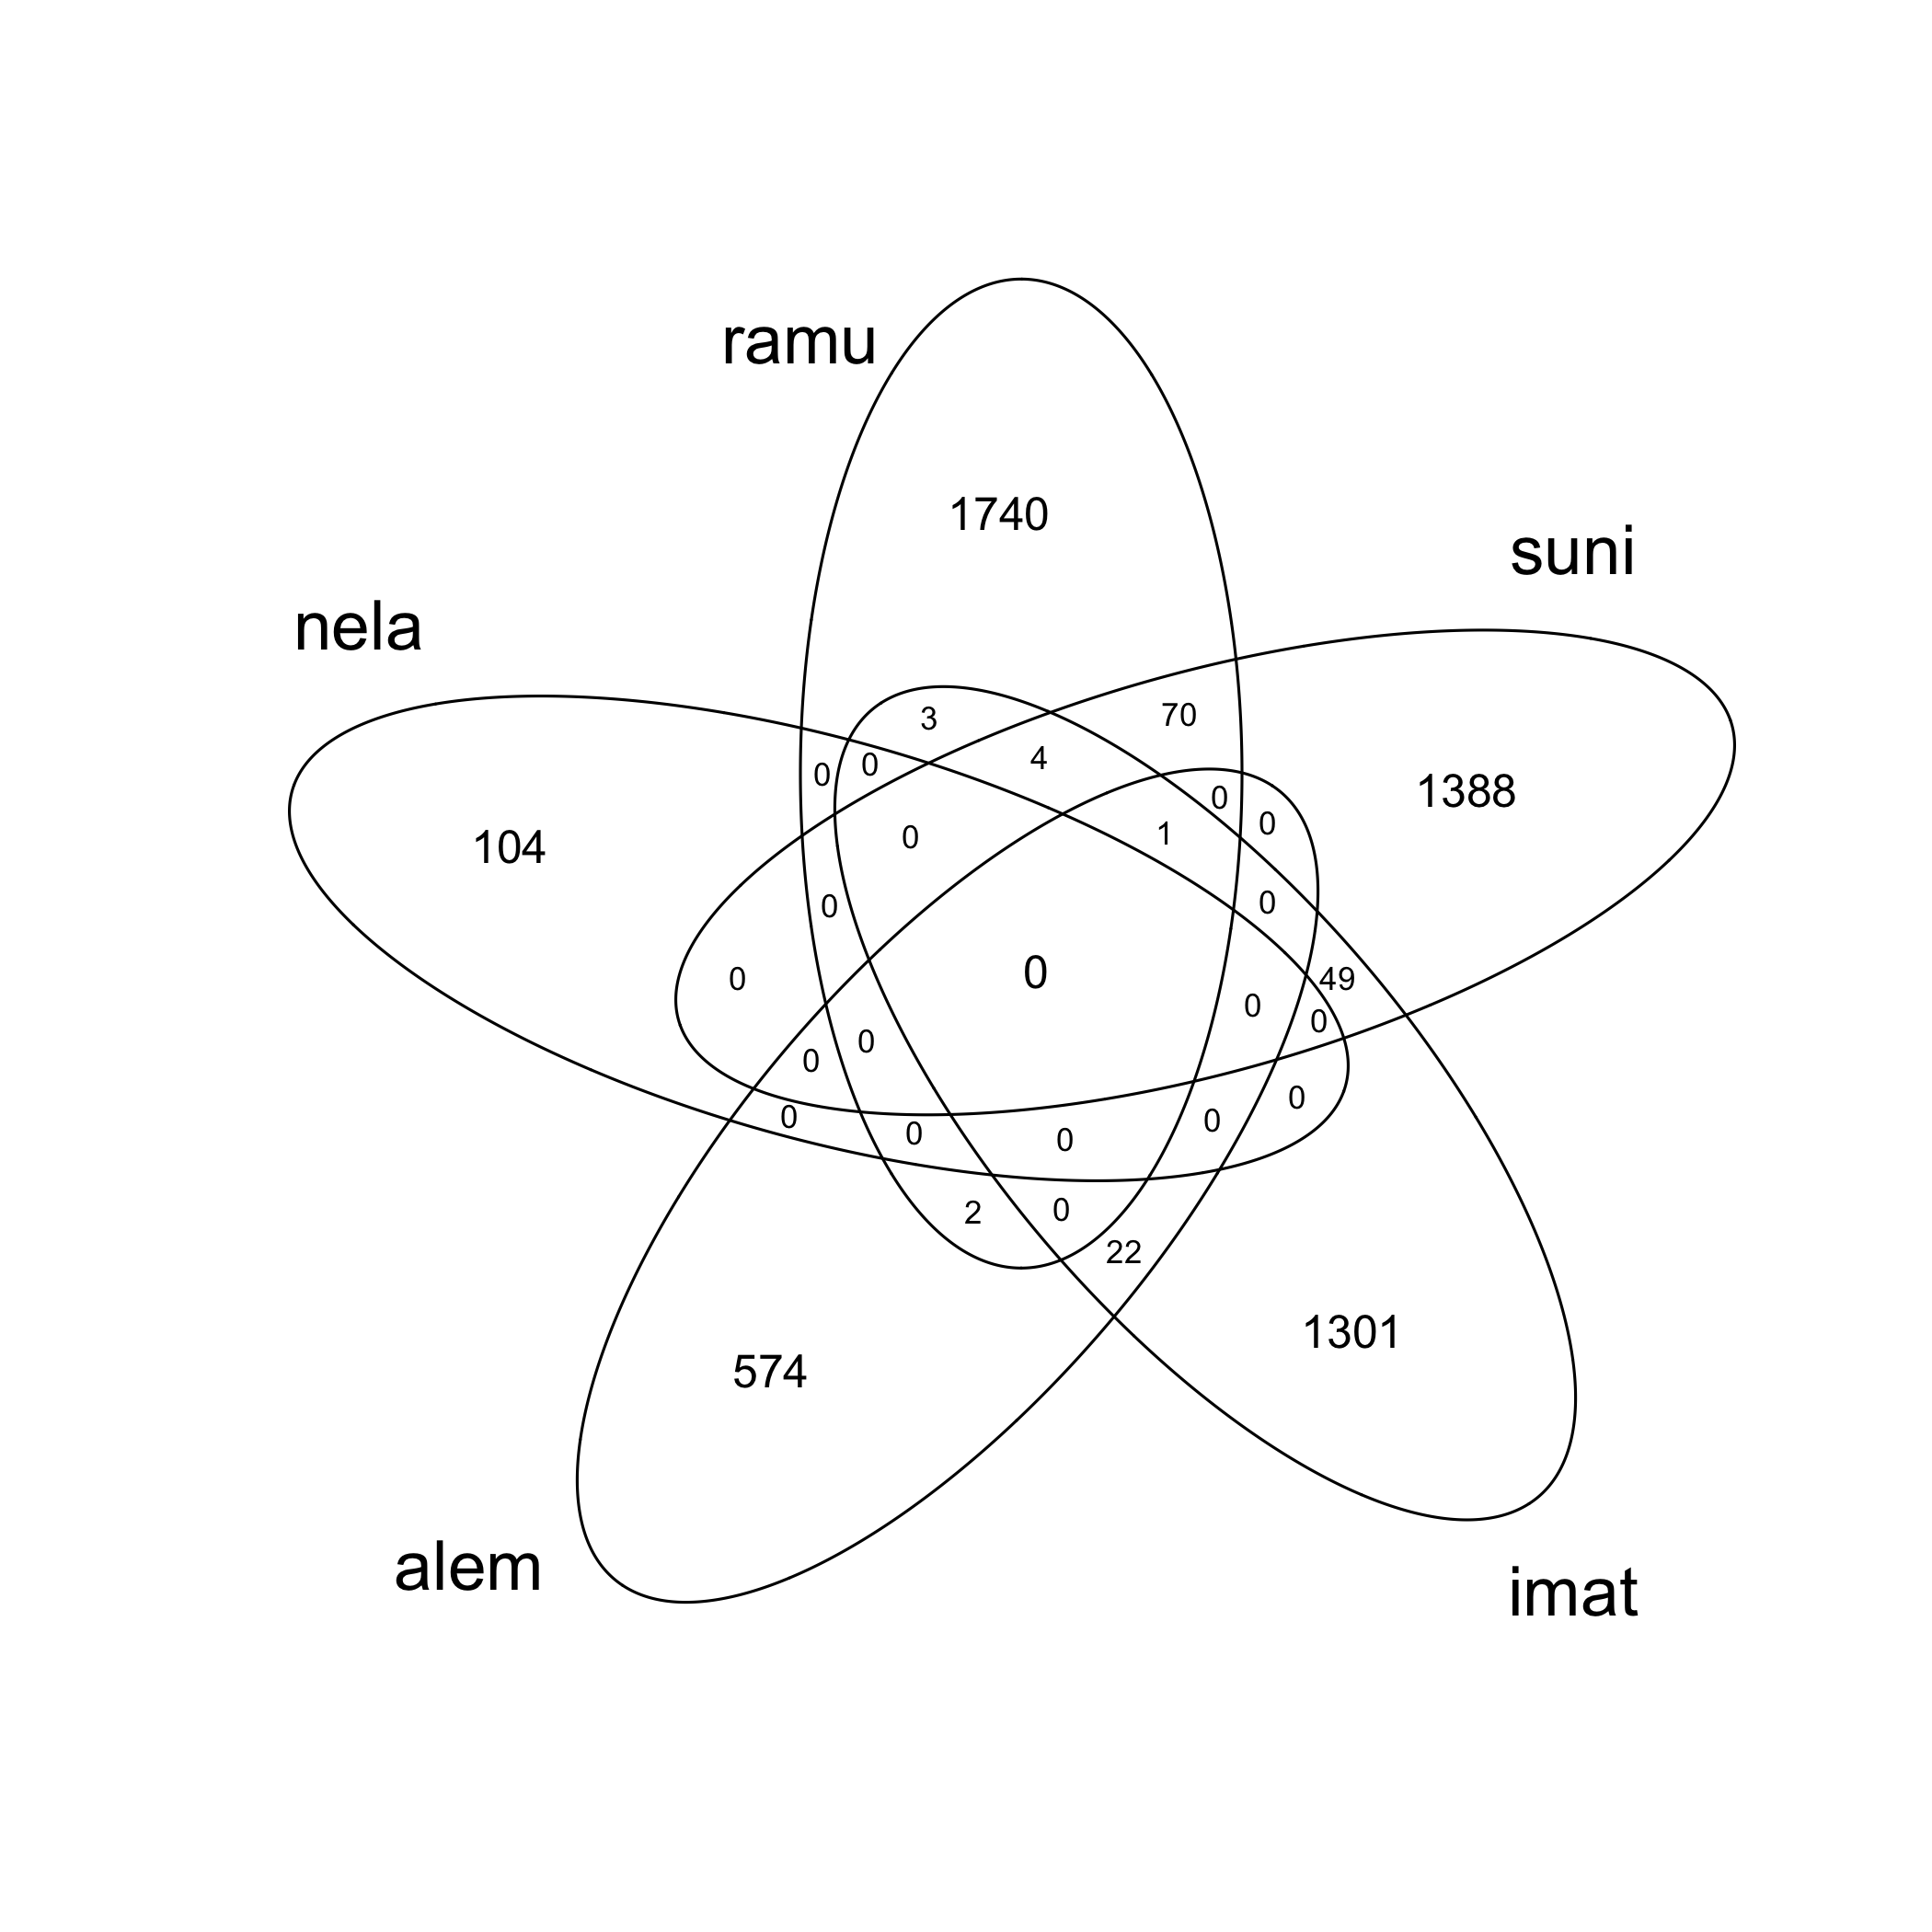
\includegraphics[scale=0.15]{citing_pmid.png}
\caption{{\bf Publications Common To First Generation References in Networks}
Intersections were calculated across all five networks for citing\_pmids (the first generation of references) and displayed as a Venn diagram.
No publications are common to all five networks. A single publication is cited in four of five networks. Abbreviations: alem (Alemtuzumab),imat (Imatinib), nela (Nelarabine), ramu (Ramucirumab), suni(Sunitinib).}
\label{fig1}
\end{figure}

\begin{figure}[!h]
\centering
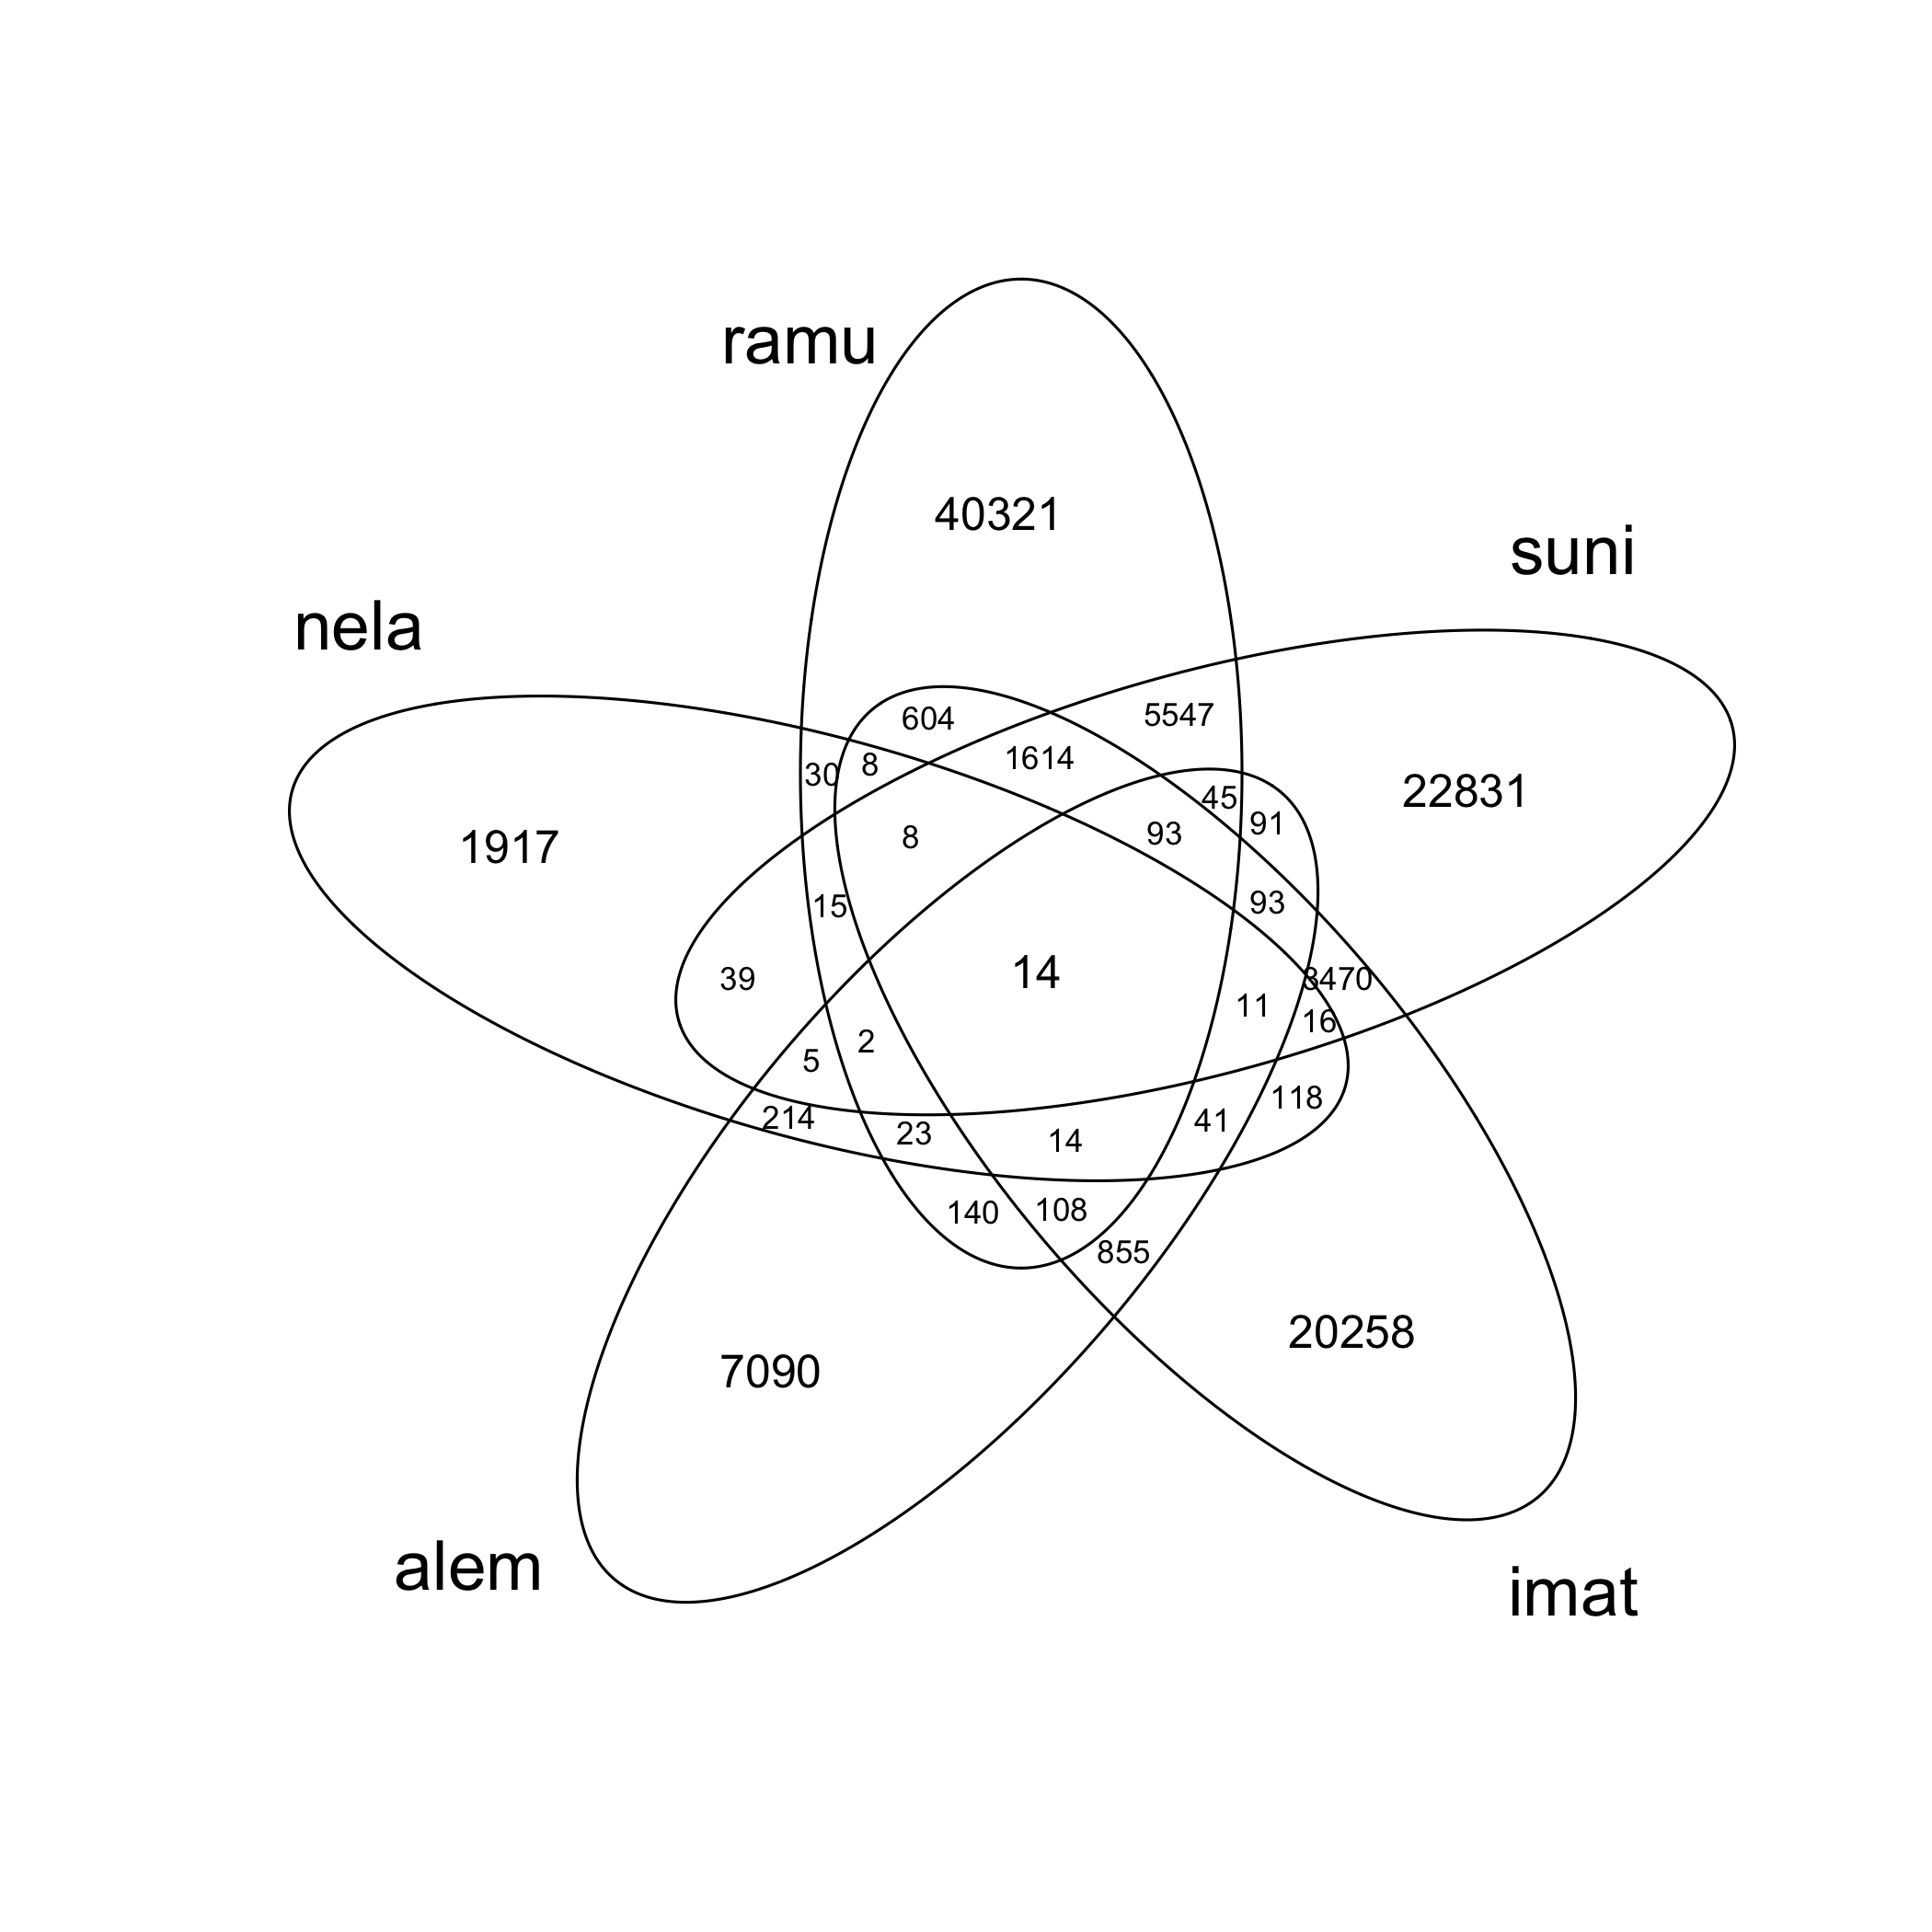
\includegraphics[scale=0.15]{cited_sid.png}
\caption{{\bf Publications Common To Second Generation References in Networks}
Intersections were calculated across all five networks for cited\_sids (the second generation of references) and displayed as a Venn diagram.
14  publications are common to all five networks. Abbreviations: alem (Alemtuzumab), imat (Imatinib), nela (Nelarabine), ramu (Ramucirumab), suni(Sunitinib).}
\label{fig2}
\end{figure}

\begin{table}[!ht]
\begin{adjustwidth}{-1.0in}{0in} % Comment out/remove adjustwidth environment if table fits in text column.
\centering
\scalebox{0.8}{\begin{tabular}{|l+l|l|l|l|l|l|l|}
\hline
%\multicolumn{4}{|l|}{\bf Heading1} & \multicolumn{4}{|l|}{\bf Heading2}\\ \thickhline
\hline
SourceYear & SourceName & Author(s) \\ 
  \hline
1958 & J. Am. Stat. Assoc. & Kaplan E.R., Meier P. \\ 
1963 & Science & Jerne, N. K. and Nordin, A. A.  \\ 
1972 & J R Stat Soc & Cox DR.  \\ 
1976 & Anal. Biochem. & Bradford MM \\ 
1977 & Br J Cancer & R. Peto, M.C. Pike, and P. Armitage  \\ 
1977 & Proc. Natl. Acad. Sci. & Sanger, F., S. Nicklen, and A.R. Coulson.  \\ 
1983 & J Immunol Methods & Mosmann T  \\ 
1984 & Adv Enzyme Regul & T.C. Chou, and P. Talalay  \\ 
1989 & Molecular Cloning: A Laboratory Manual & Sambrook, J., Fritsch, E. and Maniatis, T.  \\ 
1994 & Acta Crystallogr D & Collaborative Computational Project 4 \\ 
1994 & Acta Crystallogr. A & Navaza J.  \\ 
1997 & Cell & Levine, A. J. \\ 
1997 & Am. J. Pathol. & Perez-Atayde, A. R., Sallan, S. E., Tedrow, U., Connors, S., Allred, E., and Folkman, J.  \\ 
1998 & CA: A Cancer Journal for Clinicians & SH Landis T Murray S Bolden PA Wingo \\ 
\hline
\end{tabular}}
\vspace{2.5 mm}
\caption{{\bf Intersection of Five Networks: Second Generation Publications} Publications common to all networks at the second generation level (cited\_sid, Fig 2). } 
\label{table4}
\end{adjustwidth}
\end{table}
At the network level, 14 publications comprise the intersection of all five networks. Strikingly, not even one publication is common to all five networks at the first generation level although a single publication, the pathbreaking work of Kohler and Milstein on the production of monoclonal antibodies\cite{bibKohler}, is cited in four out of five networks. All 14 publications, the intersection of five networks, were in the second generation of citations and another 198 comprise the sum of intersections in all possible four-network combinations, roughly an order of magnitude greater than the case of cited references.  We manually grouped these 14 publications using high level descriptive terms and observed that this group was composed of  statistical methods (5 publications), molecular and cell biological methods (4 publications), analytical and structural biochemistry techniques (3 publications) and cancer biology (2 publications). Of these last two, one is a review of the p53 gene\cite{bibLevine} and the second is a study of angiogenesis in children with acute lymphoblastic leukemia\cite{bibFolkman}. Thus, the majority of this small set of 14 publications describes methods that are heavily cited in these therapeutic development networks, which is consistent with observations of the the general scientific literature \cite{bibVanNoorden}. As the subject of another study, we are actively working on a scalable automated strategy to characterize the entire dataset as well as all combinations of intersections between networks. 

With its annual budget of approximately US\$32 billion, NIH is a major funder of biomedical research. We took advantage of publicly available data\cite{bibNIHExPORTER} to identify grant support for the publications in our five networks by mapping them to pmids. A total 19,104 unique grant numbers was harvested of which 112 were found in all five networks. These awards were grouped by major type  and visualized (Fig 3.). Of note, Research Program Projects and Center grants is proportionately larger in the intersection group when compared to the total population where the proportion of research projects is larger. We speculate that the broader and collaborative nature of such awards may be more likely to result in a methods-rich population of publications than the more focused research project kind of award but further and more rigorous study is needed to elucidate this question.  The two populations of publications and grants exist in a `many to many' relationship in that each publication can acknowledge support from multiple grants and each grant can support multiple publications. Further, a significant loss of information when mapping from cited\_sid to cited\_pmid. Thus we believe that these numbers could be an underestimate of actual grant support that needs to be interpreted in the context of the false-positive and false-negative content of the publicly available data. 

\begin{figure}[!h]
\centering
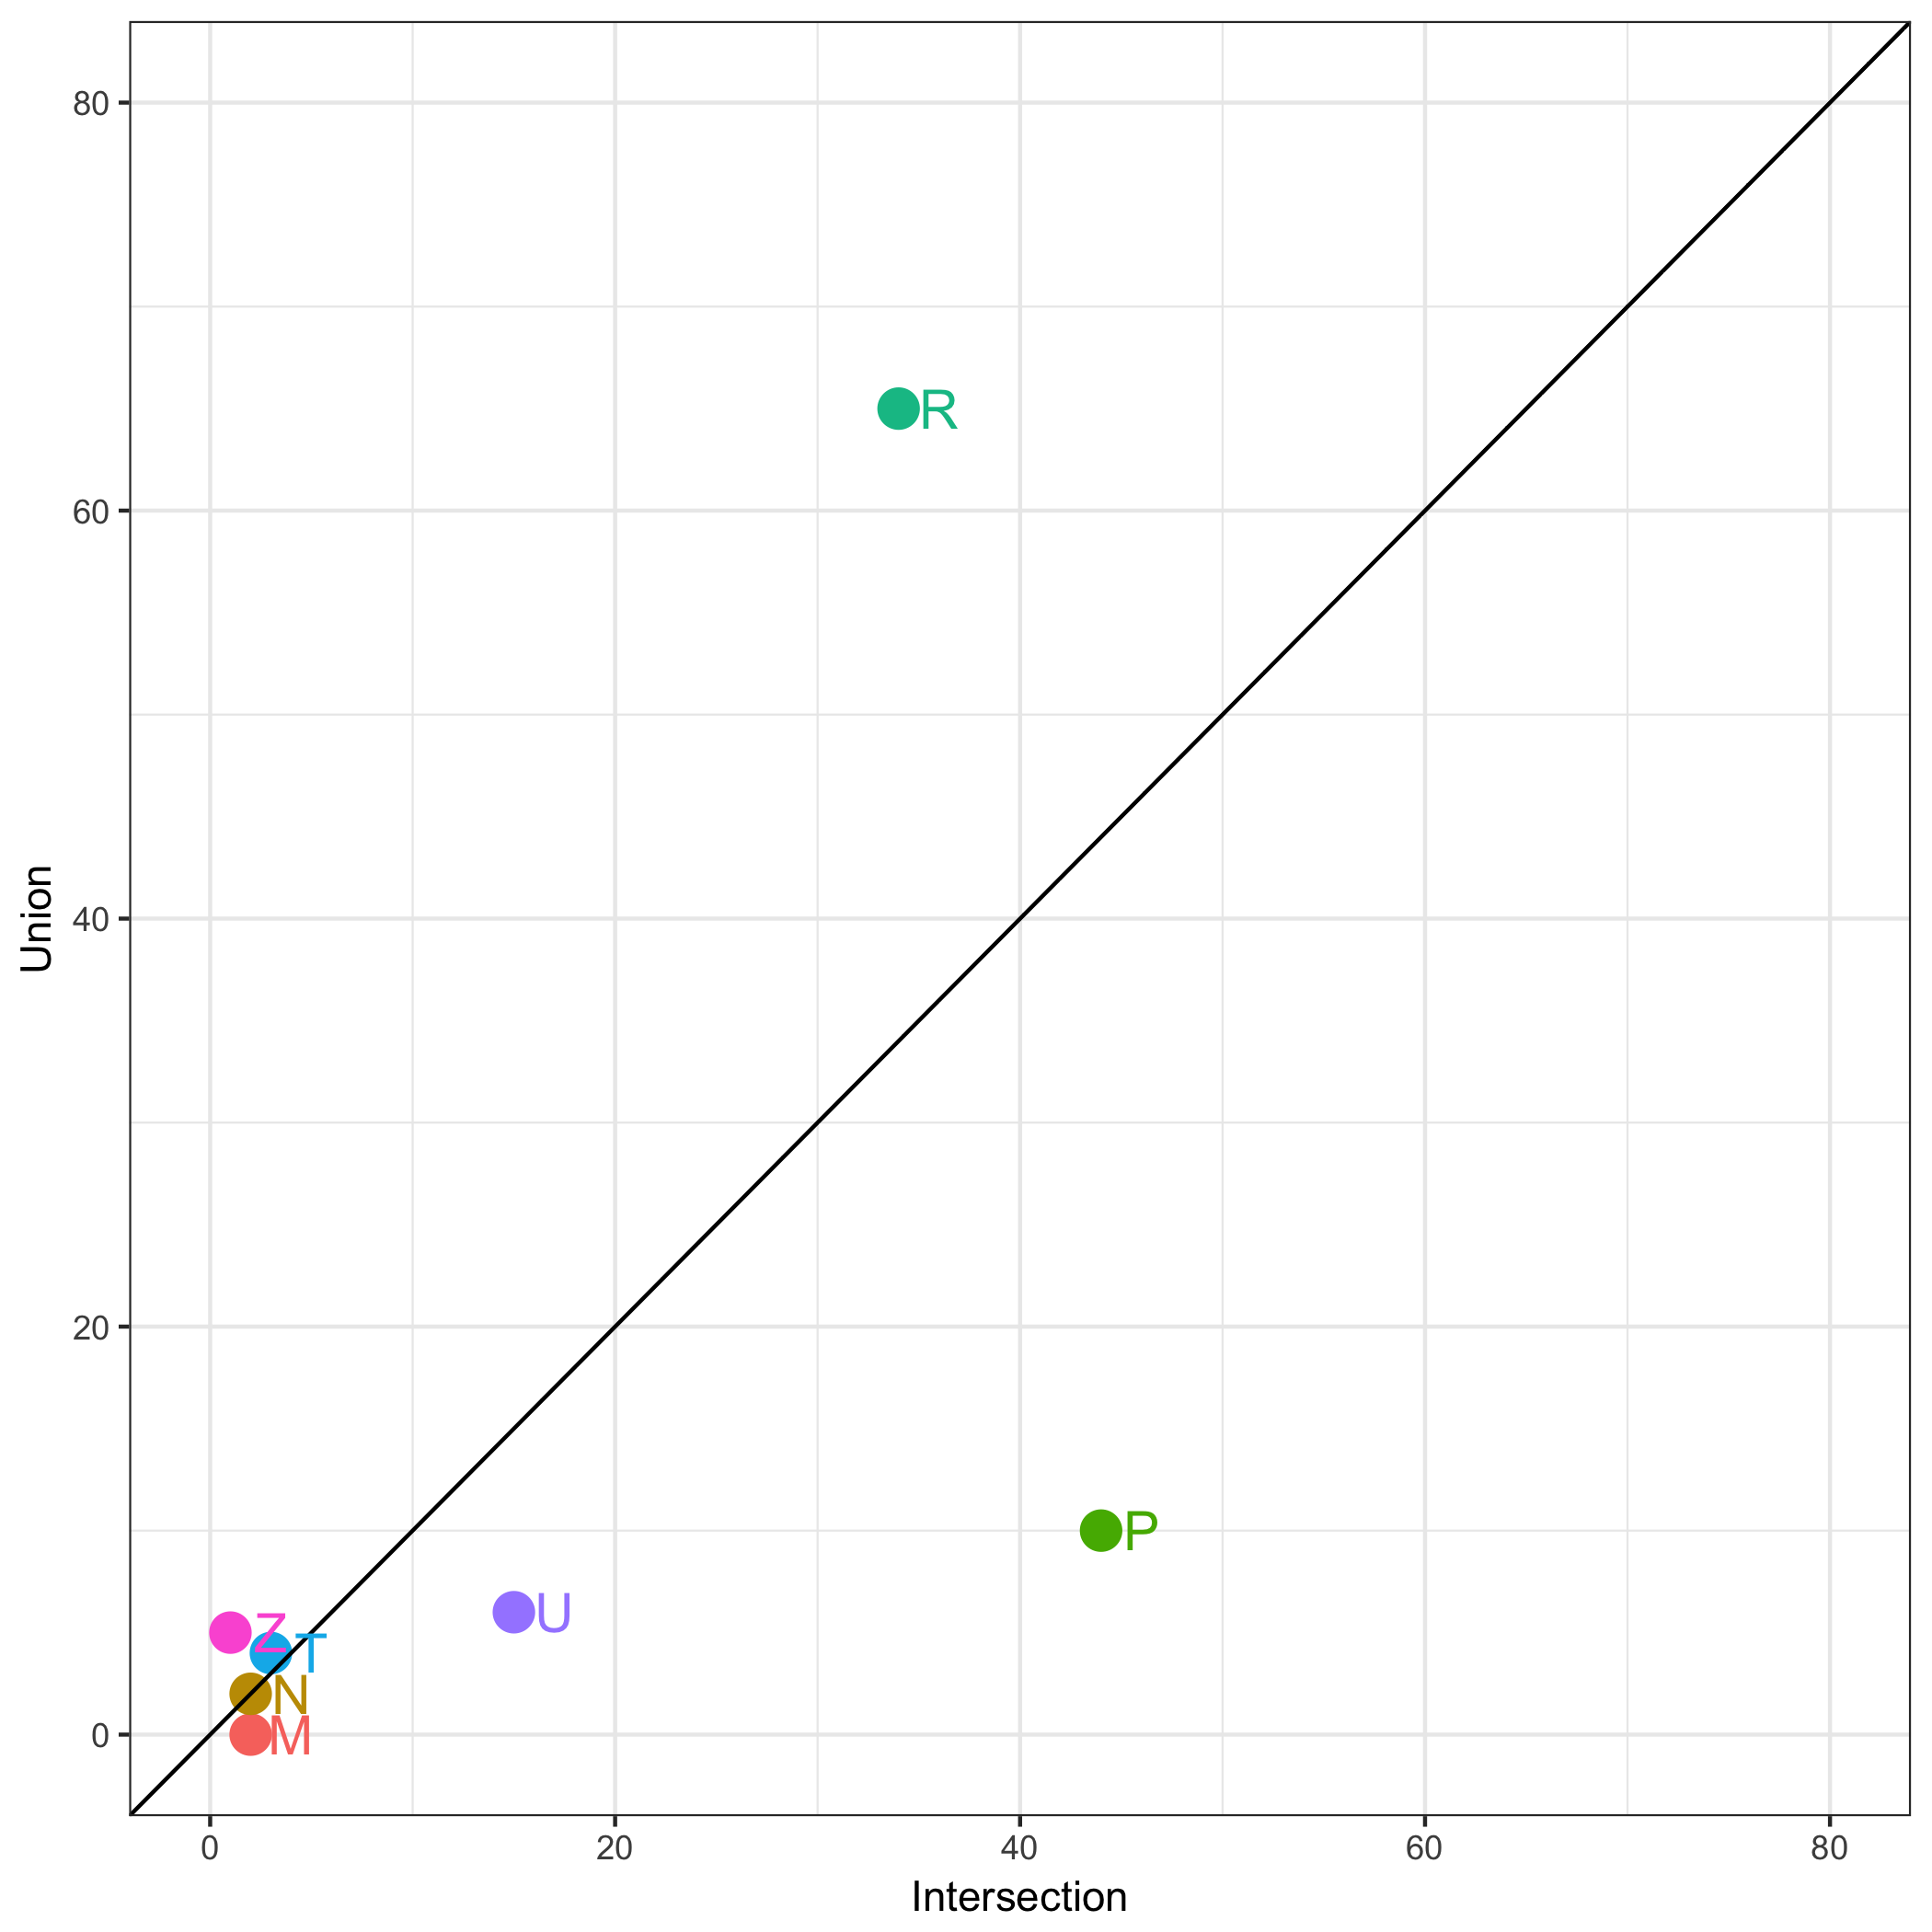
\includegraphics[scale=0.15]{proj_percent.png}
\caption{{\bf NIH Research Support} Grant and contract support for publications from NIH in the five networks was identified using ExPORTER data (Materials and Methods). 19,104 unique project numbers were identified of which 112 projects were common to all five networks. Projects were grouped by mechanism (i) P-  Research Program Projects and Centers (ii) R- Research Projects (iii) M-General Clinical Research Centers Programs (iv) N-Research and Development-Related Contracts (v) U-Cooperative Agreements (vi) T-Training Programs (vii) Z- Intramural Research. For each mechanism, the number of projects in the intersection of all five networks was plotted against the number in the union of all five networks (both expressed as percentages of their respective totals). A higher proportion of Research Program Projects and Centers awards is found in the intersection group.}
\label{fig3}
\end{figure}

Not restricted to  drug discovery and cures alone, our approach offers burden-reduction in explorations of science history, contributes to the understanding of collaboration across domains, enriches portfolio analysis, planning and optimization, and enables communications of the societal value of research. While finer critical evaluation of the content of datasets generated through this approach is perhaps best left to experts, the methodology is broadly accessible and can be viewed as another tool for citizen science.

Research support from NIH is typically made through a two stage peer-review process.  The Center for Scientific Review at NIH reviews between 50,000-60,000 grant applications each year\cite{bibBoyack}, a process involving more than 15,000 expert reviewers and individual Institutes and Centers manage smaller scale peer review operations. Thus, another layer of collaborative scientific activity preceded the awards that supported research that in turn resulted in the scientific output captured in these five networks. To describe this layer at a high-level, we matched the awards in the the five networks to the peer review panels (study sections) that evaluated them for scientific merit and calculated the intersection and union of these peer review panels. Eighty eight unique panel identifiers formed the intersection. Of these, 11 are distinguishable as Special Emphasis Panels that could be either one-time or recurring panels with temporary members, the remaining 77 are chartered panels with relatively stable membership. Some of these panels no longer exist and public records are not easily available to determine their scientific focus. For the X that could be classified (Supplemental), it is evident that they represent a rich mix of basic sciences such as chemistry, biophysics, cell biology, clinical sciences such as pathology, radiology, endocrinology. Four hundred and seven unique panel identifiers formed the union of all five networks. Of these 28 were Special Emphasis Panels, the remaining 379 panels were chartered as in the case of the intersection. These data provide evidence of broad input from invited experts in a collaborative activity that selects promising scientific projects. Assuming an average of 25 reviewers per panel (the number is likely to range from 5-40) and not considering that some of these panels are likely to have met met multiple times during the lifespan of the awards in question, a minimum of 10,000 experts comprised this additional layer of scientific regulation. We believe that the actual number is likely to be at least double.  

\section*{Supporting Information}

\paragraph*{S1 File.}
\label{S1_File}
{\bf Network Calculations} The basis of calculations for network metrics.

\paragraph*{S2 Fig.}
\label{S2_Fig}
{\bf Lorem Ipsum.} Maecenas convallis mauris sit amet sem ultrices gravida. Etiam eget sapien nibh. Sed ac ipsum eget enim egestas ullamcorper nec euismod ligula. Curabitur fringilla pulvinar lectus consectetur pellentesque.

\paragraph*{S1 Appendix.}
\label{S1_Appendix}
{\bf Lorem Ipsum.} Maecenas convallis mauris sit amet sem ultrices gravida. Etiam eget sapien nibh. Sed ac ipsum eget enim egestas ullamcorper nec euismod ligula. Curabitur fringilla pulvinar lectus consectetur pellentesque.

\paragraph*{S1 Table.}
\label{S1_Table}
{\bf Lorem Ipsum.} Maecenas convallis mauris sit amet sem ultrices gravida. Etiam eget sapien nibh. Sed ac ipsum eget enim egestas ullamcorper nec euismod ligula. Curabitur fringilla pulvinar lectus consectetur pellentesque.

\section*{Acknowledgments} %We thank Sandeep Somaiya for his support of of the nascent Netelabs concept. We thank Tandy Warnow, and Andy Chan for helpful suggestions.

\nolinenumbers
 
\begin{thebibliography}{10}

\bibitem{bibWilliams}
Williams RS, Lotia S., Holloway AK, Pico AR.
\newblock {{F}rom Scientific Discovery to Cures: Bright Stars within a Galaxy.}
\newblock Cell. 2015 Sep; 163:21--23

\bibitem{bibMaldame}
Maldame, J.
\newblock {{T}he Importance Of The History Of Science In Intellectual Formation}
\newblock Scripta Varia 2002 104:237-248

\bibitem{bibChan}
O'Shea JJ, Kanno, Y., Chan AC.
\newblock {{I}n Search of Magic Bullets: The Golden Age of Immunotherapeutics}
\newblock Cell. 2014 Mar; 157:227-240

\bibitem{bibLauer}
Lauer MS.
\newblock {{P}CSK9 Inhibitors: Lots of Work Done, Lots More to Do}
\newblock Ann Intern Med. 2016 Mar; 164(9):624-625.

\bibitem{bibFDA}
Federal Drug Administration.
\newblock {{D}rugs@FDA: FDA Approved Drug Products}
\newblock https://www.accessdata.fda.gov/scripts/cder/daf/

\bibitem{bibGooglePatents}
Google Corporation
\newblock {{G}oogle Patents}
\newblock https://patents.google.com/

\bibitem{bibNIHExPORTER}
National Institutes of Health.
\newblock {{N}IH ExPORTER}
\newblock https://exporter.nih.gov/

\bibitem{bibKohler}
K\"ohler, G., Milstein, C.
\newblock { {C}ontinuous cultures of fused cells secreting antibody of predefined specificity.}
\newblock Nature. 1975 256: 495-497

\bibitem{bibLevine}
Levine, AJ.
\newblock {{p53}, the cellular gatekeeper for growth and division.}
\newblock Cell. 1997 Feb 7;88(3):323-31.

\bibitem{bibFolkman}
Perez-Atayde AR, Sallan SE, Tedrow U, Connors S, Allred E, Folkman J.
\newblock {{Spectrum} of tumor angiogenesis in the bone marrow of children with acute lymphoblastic leukemia}
\newblock Am J Pathol. 1997 Mar;150(3):815-21.

\bibitem{bibVanNoorden}
Van Noorden R, Maher B, Nuzzo R.
\newblock {{T}he top 100 papers}
\newblock Nature 2014 514: 550-553 

\bibitem{bibBoyack}
Boyack KW, Chen M-C, Chacko G. 
\newblock {{C}haracterization of the Peer Review Network at the Center for Scientific Review, National Institutes of Health}
\newblock  PLoS One 2014 /10.1371/journal.pone.0104244


\bibitem{bibn}
Magwire MM, Bayer F, Webster CL, Cao C, Jiggins FM.
\newblock {{S}uccessive increases in the resistance of {D}rosophila to viral
infection through a transposon insertion followed by a {D}uplication}.
\newblock PLoS Gene 2011 Oct;7(10):e1002337.
\end{thebibliography}
\end{document}

